\section{The Visual Service Design Tool}
\label{sec:editor}

The first version of the VSDT has been developed as a diploma thesis~\cite{kuester2007development} in the course of the \emph{Service Centric Home} (SerCHo) project at TU Berlin in early 2007.  As the work continued it matured to a feature-rich BPMN editor with an extensible transformation framework and has already been used in a number of service orchestration scenarios in the context of a smart home environment, one of which will be shown later in Section~\ref{sec:trafo_example}.
%A rough sketch of the VSDT's architecture is shown in Figure~\ref{fig:comp}.
%
%\begin{figure}%[htbp]
%	\centering
%	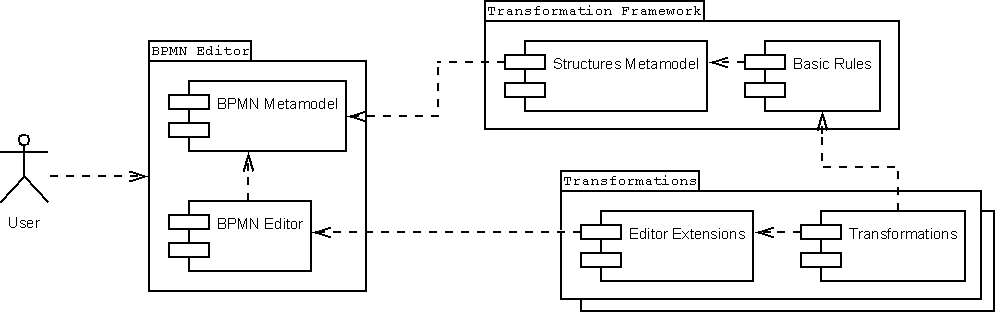
\includegraphics[width=.5\textwidth]{img/vsdt_comp.png}
%	\caption{Architecture of the Visual Service Design Tool.}
%	\label{fig:comp}
%\end{figure}

\subsection{The Metamodel}
\label{sec:editor_meta}

% Ueber die BPMN Spezifikation
The BPMN specification~\cite{omg2006business} describes in detail how the several nodes and connections constituting a BPMN diagram have to look, in which context they may be used and what attributes they have to provide.  However, it does neither give a formal definition of the syntax to be used for the metamodel, nor an interchange format, e.g.\ using an XML Schema Definition (XSD).  Thus the editor's metamodel had to be derived from the informal descriptions in the specification.
% Detaillierte Umsetzung der Spezifikation im Modell
As it was our main concern to keep as close to the specification as possible, we decided not to reuse the existing Eclipse STP BPMN Editor, which uses a simplified model of BPMN.\footnote{\url{http://www.eclipse.org/stp/bpmn/}}  Instead, almost every attribute and each constraint given in the specification has been incorporated into the metamodel, allowing the creation of any legal business process diagram.
% Sachen, wo sich das Modell von der Spezifikation unterscheidet
Still, some attributes have not been adopted in the metamodel:  For instance the possibility to model nested or even crossing Lanes has been dropped, as it turned out that this feature seems to be virtually never used in practical business process design.  Further, redundant attributes, such as the Gateway's \texttt{defaultGate} attribute, are emulated using getter methods to prevent inconsistency in the diagram model.

% StructuredBPMN-Metamodell
Concerning the transformation to BPEL and other executable languages, which in most cases are block-oriented, an extension to the usual BPMN metamodel has been designed, featuring equivalents to the basic block structures, such as sequences, decisions, parallel blocks and loops.  These elements are described in a separate metamodel, extending the editor's metamodel.  They are used only during the transformation process, especially for the mapping of the structure, as we will see in Section~\ref{sec:trafo}.


\subsection{The BPMN Editor}
\label{sec:editor_editor}

% Basis: Eclipse GMF -> Viele gute Features frei Haus
Like many others, the VSDT editor has been created using the Eclipse Graphical Modelling Framework (GMF), automatically equipping the editor with numerous features, such as support for the Eclipse properties, outline and problem view and unlimited undo and redo, just to name a few.  Being embedded in the Eclipse workbench, the editor is easy to use while at the same time providing a powerful tool for professional business architects and service developers.

% Erweiterungen: Property Sheets, Dialoge, Validierung, etc.
While GMF provides a solid basis for the editor, several customisations have been made to the code, further improving the editor's overall usability and supporting the creation of new business processes.  For example, the generated property tables have been supplemented with custom-made sheets, in which the several attributes are more clearly arranged.  For managing the non-visual elements given in the BPMN specification, such as Properties, Messages and Assignments, a number of clear and uniform dialogs has been created.  The various constraints given in the specification were translated to several audit constraints used to validate a given business process diagram.  A screenshot showing some of the editor's features can be seen in Figure~\ref{fig:screen}.

\begin{figure}%[htbp]
	\centering
	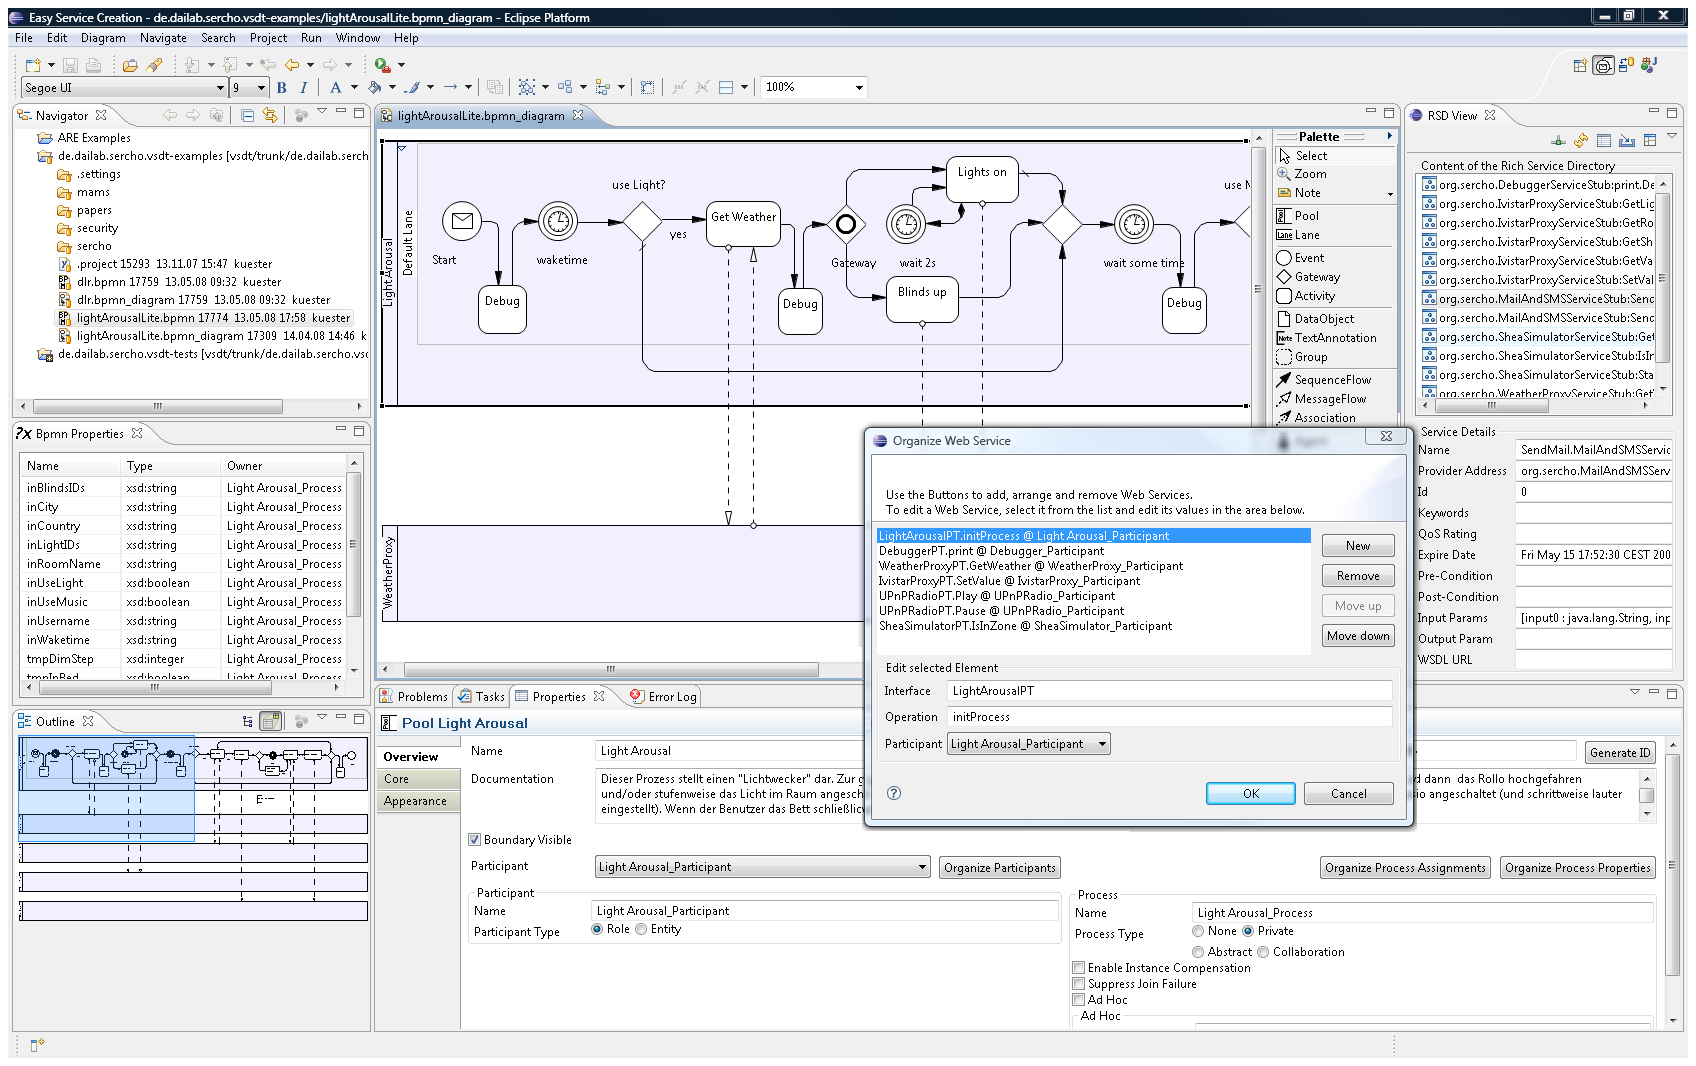
\includegraphics[width=\textwidth]{img/vsdt_080515.png}
	\caption{The Visual Service Design Tool. Clockwise: Editor view, RSD client, web services dialog, property sheet, visual outline, properties inspector, navigator.}
	\label{fig:screen}
\end{figure}

% Nachteil der Erweiterbarkeit/ BPEL-unabhaengigkeit: keine BPEL-Untertuetzung im Editor
As already mentioned, the VSDT was designed to be a pure BPMN editor and independent of BPEL, so the business process diagrams can be transformed to other languages, too, given the respective export plugins. Of course, the downside of this approach is that the editor lacks built-in support for BPEL, e.g.\ the editor itself does not validate an expression given in the diagram to conform to the BPEL syntax.  However, it is possible to supplement the editor with additional plugins, which can contribute e.g.\ to the property sheets or provide whole new views with language-specific functionality.

% Rich Service Directory
One example of how the VSDT can be extended with features specific to a certain target language --- in this case: BPEL --- is the RSD View, which can bee seen in Figure~\ref{fig:screen}, too: A client for the \emph{Rich Service Directory}, a special kind of Web service repository. Using the RSD View, existing Web services that have been registered at the RSD server can be inspected and imported into the diagram.  In the process, an Implementation object is created for the Web service as well as a set of Message objects, matching the service's input parameters and result. Optionally, also a new Pool will be created for the service, which can be connected to the currently selected Activity via a pair of Message Flows.  Further, the Implementation and the Message objects will be associated to the Activity and its type will be set to \textsc{service}.  Thus, the orchestration of existing Web services in a BPEL process can be simplified greatly.  Similar features can be created for other target languages, too.

% Export Wizards
Once the business process diagram is completed it can be validated and exported.  As the VSDT is intended to provide export features to arbitrary target languages, and to support the tool smiths in the creation of these features, we have created an elaborate export framework, which we will have a closer look at in the next section.
